%\documentclass[twocolumn]{article}
\documentclass[aps,prb,twocolumn,superscriptaddress,floatfix,longbibliography]{revtex4-2}
\setcitestyle{round,authoryear}

%\usepackage[a4paper,width=150mm,top=25mm,bottom=25mm,bindingoffset=0.6mm]{geometry}
\usepackage{amsmath,amssymb} 
\usepackage{bm}
\usepackage{graphicx} 
\usepackage{comment} 
\usepackage{textcomp}
\usepackage{subcaption}
\usepackage{float}
\usepackage{dblfloatfix}
\usepackage[title]{appendix}
\captionsetup[subfigure]{labelformat=simple,labelsep=colon}
\renewcommand{\thesubfigure}{fig\arabic{subfigure}}
%\usepackage{pdfpages}
%\usepackage{eurosym}
%\usepackage{mathtools}
%\usepackage{gensymb}

\usepackage{enumitem}
\setlist{noitemsep,leftmargin=*,topsep=0pt,parsep=0pt}

\usepackage{xcolor} % \textcolor{red}{text} will be red for notes
\definecolor{lightgray}{gray}{0.6}
\definecolor{medgray}{gray}{0.4}

\usepackage{hyperref}
\hypersetup{
    colorlinks=true,
    linkcolor=blue,
    filecolor=magenta,
    urlcolor=cyan,
}

\usepackage[noabbrev,capitalize,nameinlink]{cleveref}
\urlstyle{same}


% Code to add paragraph numbers and titles
\newif\ifptitle
\newif\ifpnumber
\newcounter{para}
\newcommand\ptitle[1]{\par\refstepcounter{para}
{\ifpnumber{\noindent\textcolor{lightgray}{\textbf{\thepara}}\indent}\fi}
{\ifptitle{\textbf{[{#1}]}}\fi}}
\ptitletrue  % comment this line to hide paragraph titles
\pnumbertrue  % comment this line to hide paragraph numbers

% minimum font size for figures
\newcommand{\minfont}{6}

% Uncomment this line if you prefer your vectors to appear as bold letters.
% By default they will appear with arrows over them.
% \renewcommand{\vec}[1]{\bm{#1}}

% Allows to rewrite the same title in the supplement
\newcommand{\mytitle}{Protoplanetary Discs around Low Mass Stars:\\ The effect of the Temperature on the Disc Structure}

\begin{document}

\title{\mytitle}

\author{Adam Parkosidis}
\email[]{adam.parkosidis@student.uva.nl}
\affiliation{Jeremiah Horrocks Institute for Mathematics, Physics \& Astronomy, University of Central Lancashire, Preston PR1 2HE, UK}

%\date{\today}

\begin{abstract}
Planets form in young protoplanetary discs that are made of gas and dust. We simulate locally isothermal gaseous protoplanetary discs evolving around low mass stars using the SPH code ``PHANTOM'' while varying the disc-to-star mass ratio and the initial exponent of the temperature profile. We investigate different temperature profiles and different disc-to-star mass ratios to estimate the surface density profile of the disc when it reaches the equilibrium state.  We refer to the period before this point as the time taken for the discs to relax (approximately few $kyrs$). Each simulation evolves for $5000yr$, which corresponds to 5 orbits of the outer radius of the disc. The disc-to-star mass ratio,$w$, is set to $0.01, 0.05$ and $0.1$, while the temperature profile follows a power law $T_{disc} \propto r^{-q}$(\cite{armitage2020astrophysics}). We find that the transport of angular momentum towards the disc outer region is more efficient in colder discs, thus discs with steeper initial temperature profile result to steeper surface density profile when they reach the equilibrium state. Furthermore we find that more massive systems-more massive discs around more massive stars- also result to steeper surface density profile after they have relaxed. Surprisingly, we find that the aforementioned behavior does not apply in the case of the least massive star ($M_{\star}=0.2M_{\odot}$). Furthermore, we see that this discrepancy becomes greater for bigger values of $w$ corresponding to more massive discs around the star. 
\end{abstract}
\maketitle


\section{Introduction}
Molecular clouds of gas and dust in the Galaxy collapse under their own gravity when their mass exceeds the Jean mass creating stars with non-zero initial angular momentum and substantial gaseous protostellar discs around them (\cite{shu1987star}). In this early stage, for low mass stars, the disc mass is expected to be comparable to that of the protostar, as a result the self-gravity of the disc should influence the evolution of the system playing an important role in the creation of planets or low mass stars via disc fragmentation (\cite{boss1997giant}), as well as affect the accretion of mass onto the protostar's surface. Protostellar discs are also commonly referred as protoplanetary discs and even though there is no strict separation between their definitions, discs  with mass comparable to the star mass tend to be referred to as ``protostellar'', $w \geq 0.1$, while discs with $w < 0.1$ as ``protoplanetary''.

Protoplanetary discs have masses from $10^{-3}M_{\odot}$ to $10^{-1}M_{\odot}$, radii from $10 AU$ to $10^{3}AU$ and lifetimes less than $10$Myr. Such discs are common around PMS stars and are perceived by the strong far-IR/submillimeter radiation they emit, while the accretion of their material onto the central star produces also UV radiation. The evolution of the so called protoplanetary discs is determined by the combined effects of the star's gravity and irradiation, and the angular momentum processes in the disc.

\section{Hydrodynamic Simulations}
\subsection{PHANTOM}
We carry out different smoothed particle hydrodynamic (SPH) simulations using PHANTOM code (\cite{price2018phantom}) to evaluate the slope of the surface density profile for locally isothermal gaseous discs after they have reached the relaxed state. The simulations consist of $N = 200,000$ particles initially distributed from $r_{in} = 1 AU$ to $r_{out} = 100 AU$. We assume that they have the same mass
\begin{equation}\label{eq:particle mass}
    m_i = \frac{M_{disc}}{N}
\end{equation}
The duration of each simulation is $5000$yr corresponding to $5$ orbits of the disc outer radius.  As the system evolves angular momentum is transferred outwards, while mass inwards. Gas particles that fall within the region of $r <r_{in}$ accreted onto the central star, represented here as a point mass. The viscous evolution process is modeled using the SPH artificial viscosity $a_{AV}=0.1$ corresponding to discs with
\begin{equation}\label{eq:artificial viscosity}
    a_{SS} = \frac{a_{AV}}{10} \frac{<h>}{H}
\end{equation}
where $a_{SS}$ is the Shakura \& Suynaev parameter (\cite{shakura1973black}, \cite{lodato2011smoothed}), $H$ is the scale height and $<h>$ is the mean smoothing length on particles in a cylindrical ring at a given radius. For locally isothermal discs where the temperature of the gas is prescribed as a function of position and assuming an ideal gas, the equation of state is
\begin{equation}\label{eq:equation of state}
    P = \frac{\rho k_{\beta}T}{\mu m_H} = c_s^2 \rho
\end{equation}
where $P$ is the pressure, $\rho$ the density of the gas and $c_s$ the sound speed. 
Following (\cite{lodato2007warp}) the parametrisation of the sound speed $c_s$ is
\begin{equation}\label{eq:sound speed}
    c_s = c_{s,0}R^{-q_c}
\end{equation}
where $c_{s,0}$ determines the disc thickness (is calculated at a reference radius, in our case $R_{ref} = 10 AU$) and the height scale $H$ is
\begin{equation}\label{eq:height scale}
    H = \frac{c_s}{\Omega_K} = \frac{c_{s,0}}{\sqrt{GM_\star}} R^{\frac{3}{2}-q_c}
\end{equation}
from which $c_{s,0}$ can easily be determined for a given $R=R_{ref}$. 
From \eqref{eq:equation of state}, \eqref{eq:sound speed} and \eqref{eq:height scale} the sound speed profile is given by
\begin{equation}
    c_s(R) = \sqrt{\frac{k_{\beta}T_{ref}}{\mu m_H}} R_{ref}^{q_c} R^{-q_c}
\end{equation}
At this point we performed several test simulations, varying the reference radius between values close to $r_{in}$ and figured out that the result on the slope of the density profile is negligible.
\section{Initial Conditions}
 We set the initial disc density, temperature and rotational velocity using information from theoretical models and observations. The temperature and surface density exponents, disc mass and radius and as well as star mass are free parameters. In this section we describe the initial conditions in detail.

\subsection{Disc Volume and Surface Density}
Steady-state theory suggests that the surface density of an accretion disc follows a power law of the form $\Sigma (r) \propto r^{-p}$ (\cite{armitage2020astrophysics}), where $r$ the distance from the central star on the disc mid-plane. Furthermore, semi-analytical studies of collapsing rotating cloud cores indicate that $p$ is between $1$ and $\frac{3}{2}$  (\cite{lin1990formation}). In our work we assume a surface density profile
\begin{equation}\label{eq:surface density}
    \Sigma (R) = \Sigma_0 (\frac{R_0^2}{R_0^2 + R^2})^{p/2}
\end{equation}
where $\Sigma_0$ is the surface density at $r=0$, $R_0 = 10 AU$ is the softening radius, which is used to prevent surface density from getting nonphysically large near the star, and $R$ denotes the distance from the star on the disc mid-plane. We note that if $x-y$ is the disc mid-plane then $R=\sqrt{x^2 + y^2}$, while $r=\sqrt{x^2 + y^2 +z^2}$ denotes the distance from the star in three dimensions. In our models we select $p=2.05$. We compared the initial surface density profile with different values of $p$ to the surface density profile at 1000 years and found that a steeper (higher $p$) profile matched the relaxed state better. This would mean that the simulation takes less time to reach that relaxed state which is important for us, because discs fragment very quickly (few thousand years)  and we can only ``trust'' the simulation after the disc is relaxed.

The total mass of disc is obtained from 
\begin{equation}\label{eq:mass}
    M(R) =\int_{R_{in}}^{R_{out}} \Sigma (R) 2 \pi R \,dR \
\end{equation}
where there is a gap in the disc around the central star and $R_{in}$ is the inner radius of the disc, while $R_{out}$ is the external one. From \eqref{eq:surface density} and \eqref{eq:mass} is derived that
\begin{equation}
    M_{disc} = \frac{2 \pi R_{0}^2}{2-p} [(\frac{R_{0}^2 + R_{out}^2}{R_{0}^2})^{1-\frac{p}{2}}) - (\frac{R_{0}^2 + R_{in}^2}{R_{0}^2})^{1-\frac{p}{2}}]
\end{equation}
The vertical density profile is estimated be taking into account the hydrostatic equilibrium in the direction vertical to the disc mid-plane ($z$-direction). We assume that the disc is Keplerian and the  vertical component of the gravitational acceleration, $g_z$ must balance the vertical pressure gradient
\begin{equation}\label{eq:vertical equilibrium}
    \frac{1}{\rho} \frac{dP}{dz} = -g_z = -\Omega^2z
\end{equation}
We also consider the effect of self-gravity of the disc, thus we modify \eqref{eq:vertical equilibrium} and we adopt
\begin{equation}\label{eq:vertical equilibrium self gravity}
    \frac{1}{\rho} \frac{dP}{dz} = -g_z = -(\frac{G(M_{\star} + M_{disc}(<R))}{R})z + g^D_z
\end{equation}
where $M_{disc}(<R)$ is the mass of the disc interior to radius $R$ and $g_z$ the self-gravity of the disc in the $z$-direction. We therefore assume that the radial component of the disc self gravity can be approximated by considering that the disc mass within radius $R$ is located in the position of the star. From \eqref{eq:equation of state}, \eqref{eq:vertical equilibrium self gravity} and assuming that the disc is geometrically thin ($z << R$) the volume density of the disc is given by a Gaussian
\begin{equation}\label{eq:volume density}
    \rho(R,z) = \rho (R,0)e^{\frac{-z^2}{2H^2}}
\end{equation}
where $\rho (R,0)$ is the density midplane and can be calculated from the surface density
\begin{equation}\label{eq:surface volume density}
    \Sigma (R) = \int_{-\infty}^{\infty} \rho(R,z) \,dz\ = \sqrt{2 \pi}H(R)\rho(R,0)
\end{equation}
In case of a self-graviting disc with a central star (\cite{bertin1999astronomy}) the scale height $H(R)$ is given by 
\begin{equation}\label{eq:scale height self gravity}
    H(R) = \sqrt{\frac{\pi}{8}} \frac{c_s(R)}{\Omega(R)}(\sqrt{\frac{1}{Q(R)^2}+ \frac{8}{\pi}}- \frac{1}{Q(R)})
\end{equation}
where $Q(R)$ is the Toomre parameter.

Finally, from \eqref{eq:volume density} and \eqref{eq:surface volume density} we obtain 
 \begin{equation}\label{eq:volume density extended}
     \rho (R,z) = \frac{\Sigma(R)}{\sqrt{2 \pi}} \frac{1}{H(R)} e^{\frac{-z^2}{2H(R)^2}}
 \end{equation}
which is the adopted volume density profile for the simulations.

\subsection{Disc Temperature}
The two major physical processes that heat the disc are irradiation from the central star and energy generated by viscous dissipation within the disc. Discs that just absorb and re-emit radiation from the central star ({\it passive discs}) follow a temperature profile $T_{d} \propto r^{-\frac{3}{4}}$ (assuming a geometrically thin disc, \cite{armitage2020astrophysics,adams1986infrared}). Simultaneously, discs that produce heat by viscous dissipation within the disc ({\it active discs}) also follow a temperature profile $T_{d} \propto r^{-\frac{3}{4}}$ (\cite{friedjung1985accretion}). The difference is that for passive discs the luminosity of the central star determines the proportionality constant, while for active discs it is determined by the mass accretion rate and the mass of the central star. However, observations show flatter temperature profiles, which suggest even hotter discs. \cite{kenyon1987spectral} concluded that this could be explained if discs are flared (the thickness of the disc increases as the distance from the star increases) rather than flat. In that case the temperature profile is not that steep, $T_{d} \propto r^{-\frac{1}{2}}$, while they showed that in small radii a flared disc temperature profile could be described by $T_{d} \propto r^{-\frac{3}{4}}$ (isothermal flared disc diverges from the flat solution at $\frac{r}{R_{\star}} \approx 3$). Other solutions have also been proposed. \cite{natta1993temperature} pointed out that even a small amount of dust  distributed above the disc will scatter considerable amount of radiation back towards the disc mid-plane heating the disc, while \cite{chiang1997spectral} assumed a model in which outer parts of the disc are optically thin, forming a ``disc atmosphere''. As a result, dust grains in the atmosphere absorb unattenuated radiation from the star and become hotter, creating a superheated region in the outer regions of the disc. In our work we assume a general profile for the disc temperature
\begin{equation}\label{eq:temperature profile}
    T_{d}(R) = \left(T_0^{2}(\frac{R^2 + R_0^{2}}{AU^2})^{-q} + T_{\infty}^2\right)^{\frac{1}{2}}
\end{equation}
where $R_0 = 0.25 AU$ is the softening radius that prevents temperature to be infinitely large close to the center of the star, $T_0$ is the temperature at $r=1AU$ (provided that $R_0 << 1AU$, which is generally true), $T_{\infty} = 10 K$ is the temperature far away from the star and from \eqref{eq:sound speed}, \eqref{eq:equation of state} and \eqref{eq:temperature profile} it is evident that $q=2q_c$. \cite{beckwith1990survey} and \cite{osterloh1995millimeter} observed 81 and 121 young PMS stars in the Tau-Aur dark cloud respectively and found values of $q$ from $0.35$ to $0.8$.  We consider different exponents for our models as $q$ equals to $0.3$, $0.5$ and $ 0.7$ modifying the disc temperature profile.

\subsection{Disc Rotation}
To calculate the initial disc velocity of the disc at distance $R$ we assume that all particles of the disc at the same distance $R$ have the same velocity $u$, independently of the distance $z$ from the mid-plane. Even though we assumed a Keplerian disc, we slightly modify the equation of the velocity to include the effect of self-gravity
\begin{equation}\label{eq:rotational velocity}
    u(R) = \left(\frac{G(M_{\star} + M_{disc}(<R))}{R}\right)^\frac{1}{2}
\end{equation}
where $M_{disc}(<R)$ is the mass of the disc interior to radius $R$. From \eqref{eq:rotational velocity} it is obvious that a less massive disc tends to rotate with keplerian velocity due to the fact that its self-gravity is negligible compared to the gravity of the star, in contrast a more massive disc rotates faster than a purely keplerian disc, because of the effect of self gravity.

\section{Determination of Free Parameters}
First of all we set the initial values for free parameters that are critical for our simulations. More specifically we set the initial mass for the central star, $M_{\star}$, and the disc, ($M_{disc}$), based on theoretical models and observations, we also calculate the temperature ($T_0$) at distance $R=1AU$ from the star and finally we select the exponent, $q$, which determines the slope of the disc temperature profile .

At this point we need an estimation about $T_0$, thus we adopt a very simple model: we assume a flat thin disc in the equatorial plane that absorbs all the incident stellar radiation and re-emits it as a single temperature blackbody, while we neglect other heating processes (e.g energy generated by viscous dissipation within the disc).

The star is assumed to irradiate as a spherical blackbody with $R_{\star} =1 R_{\odot} $, thus the flux $F_{\star}$ passing through its surface is
\begin{equation}\label{eq:flux}
  F_{\star}=\sigma T_{\star}^4
\end{equation}
where $\sigma$ is {\it Stefan-Boltzmann constant}, the total intensity for such an emitter is
\begin{equation}\label{eq:total intensity}
    I_{\star} = \frac{F_{\star}}{\pi} = \frac{\sigma T_{\star}^4}{\pi}
\end{equation}
while the luminosity $L{\star}$ for a spherical star is
\begin{equation}\label{eq:luminosity}
  L = 4\pi R_{\star}^2 F_{\star}
\end{equation}
Therefore from \eqref{eq:flux} and \eqref{eq:luminosity} we obtain
\begin{equation}\label{eq:luminosity2}
  L = 4 \pi R_{\star}^2 \sigma T_{\star}^4
\end{equation}

We also consider a point at an arbitrary distance $r$ from the star, from the point's position, the star subtends a solid angle $ \frac{\pi R_{\star}^2}{r^2}$ (\cite{urry1995unified}) and the total intensity towards it is $I_{\star}$. As a result from \eqref{eq:total intensity} and \eqref{eq:luminosity2} the total flux passing through this surface is
\begin{align}
    F = \frac{1}{4} \int_{\Omega}^{} I_{\star} \,d_{\Omega}\ \\
    F = \frac{1}{4} \frac{\pi R_{\star}^2}{r^2} I_{\star}\\
    16\sigma T(r)^4 = \frac{4 \pi R_{\star}^2}{r^2} \frac{\sigma T_{\star}^4}{ \pi} \\
    T(r) = (\frac{L_{\star}}{16 \pi \sigma r^2})^{1/4} \label{eq:temperature-distance}
\end{align}
Now we can estimate the luminosity of the star based on the {\it mass-luminosity relation}, which indicates that
\begin{equation}\label{eq:mass-luminosity relation}
  \frac{L}{L_{\odot}} = a(\frac{M_{\star}}{M_{\odot}})^{n}
\end{equation}
with $n$ depending on the mass of the star. Empirical data from observations provide
\begin{table}[!htbp]
\centering
  \begin{tabular}{ccc}
  \hline
  \textbf{Initial Mass} $M_{\odot}$ & \textbf{Index n} & \textbf{Constant a}\\
  \hline \hline
  $0.2 < M_{\star} < 0.43$ &  2.5 & $a \cong 0.1849$\\
  $0.43 < M_{\star} < 2$ &  4.5 & $a = 1$\\
  $2 < M_{\star} < 55$ &  3 & $a \cong 2.8284$\\
  \hline
  \end{tabular}
 \caption{Index n in different mass regimes}\label{tab:mass-luminosity}
\end{table}

while for even bigger stellar masses $n \cong 1$ and $a \cong 3025$ (\cite{alma991001241309703821}).

Typical values for the disc mass ranging from $10^{-3}M_{\odot}$ to $10^{-1}M_{\odot}$. In our work we assume low mass stars, thus from \eqref{eq:temperature-distance} and \eqref{eq:mass-luminosity relation} we calculate the temperature $T_0$ at distance $r=1 AU$. At this point it is critical to mention that even though the calculation of temperature profile did not derived from sophisticated computations, it is a good enough approximation for our model. The results of our calculations are presented in \cref{tab:star related initial conditions}.
\begin{table}[ht]
\centering
  \begin{tabular}{ ccc}
  \hline
   M$_{\star} \; (M_{\odot})$ & $L_{\star} (L_{\odot}$) &$T_{0} \; K$\\
  \hline \hline
  0.2  & $3.31 \times 10^{-3}$ & 70\\
  0.6 & $10^{-1}$ & 160\\
  1 & $1$ & 280\\
  \hline
  \end{tabular}
\caption{Star related initial input parameter: Mass, Luminosity and Temperature at distance 1 AU}\label{tab:star related initial conditions}
\end{table}

We have now determined the necessary quantities that are implemented in our model. In \cref{tab:initial conditions} we present the initial conditions for each simulation.
\section{Results}
To analyse and visualize the output data of each simulation we use the ``Plonk" Python library (\cite{2019JOSS....4.1884M}). We present 1-D (\cref{app:appendixA}) and 2-D (\cref{app:appendixB}) illustrations of the surface density of the disc for each simulation in pursuant to  \cref{tab:initial conditions}. The figures are positioned in $3 \times 3$ blocks based on the star mass of 

\begin{table}[!htbp]
  \centering
  %\setlength{\tabcolsep}{20pt} % Default value: 6pt
  \begin{tabular}{cccccc}
  \hline
  $Run$ & $M_{\star} \; (M_{\odot})$ & $M_{disk} \; (M_{\odot})$ & $w$ & $T_0 \; (K)$ & q \\
  \hline \hline
  1 & 0.2 & 0.002 & 0.01 & 70 & 0.3 \\
  2 & 0.2 & 0.002 & 0.01 & 70 & 0.5 \\
  3 & 0.2 & 0.002 & 0.01 & 70 & 0.7 \\
  \hline
  4 & 0.2 & 0.01 & 0.05 & 70 & 0.3 \\
  5 & 0.2 & 0.01 & 0.05 & 70 & 0.5 \\
  6 & 0.2 & 0.01 & 0.05 & 70 & 0.7 \\
  \hline
  7 & 0.2 & 0.02 & 0.1 & 70 & 0.3 \\
  8 & 0.2 & 0.02 & 0.1 & 70 & 0.5 \\
  9 & 0.2 & 0.02 & 0.1 & 70 & 0.7 \\
  \hline
  10 & 0.6 & 0.006 & 0.01 & 160 & 0.3 \\
  11 & 0.6 & 0.006 & 0.01 & 160 & 0.5 \\
  12 & 0.6 & 0.006 & 0.01 & 160 & 0.7 \\
  \hline
  13 & 0.6 & 0.03 & 0.05 & 160 & 0.3 \\
  14 & 0.6 & 0.03 & 0.05 & 160 & 0.5 \\
  15 & 0.6 & 0.03 & 0.05 & 160 & 0.7 \\
  \hline
  16 & 0.6 & 0.06 & 0.1 & 160 & 0.3 \\
  17 & 0.6 & 0.06 & 0.1 & 160 & 0.5 \\
  18 & 0.6 & 0.06 & 0.1 & 160 & 0.7 \\
  \hline
  19 & 1 & 0.01 & 0.01 & 280 & 0.3 \\
  20 & 1 & 0.01 & 0.01 & 280 & 0.5 \\
  21 & 1 & 0.01 & 0.01 & 280 & 0.7 \\
  \hline
  22 & 1 & 0.05 & 0.05 & 280 & 0.3 \\
  23 & 1 & 0.05 & 0.05 & 280 & 0.5 \\
  24 & 1 & 0.05 & 0.05 & 280 & 0.7 \\
  \hline
  25 & 1 & 0.1 & 0.1 & 280 & 0.3 \\
  26 & 1 & 0.1 & 0.1 & 280 & 0.5 \\
  27 & 1 & 0.1 & 0.1 & 280 & 0.7 \\
  \hline
  \end{tabular}
\caption{The initial conditions of each simulation.}\label{tab:initial conditions}
\end{table}
the system and every column corresponds to the initial value of the $q$ exponent with $|q|=0.3, 0.5, 0.7$ respectively.
The fitting curve process indicates a power law (\cref{app:appendixA}) for the surface density profile
\begin{equation}
    \Sigma(R) = \Sigma_0 R^{-p}
\end{equation}\label{eq:final surface density profile} and the parameters of the fit are presented in \cref{tab:final slopes}.
Due to the fact that we are interested in the slope of the surface density profile of the disc the 1-D illustrations have been plotted for $20 AU< R < 50AU$, where the approximation of a straight line in logarithmic scale is very good. Each graph consists of $100$ points, thus the disc has been divided to $100$ annuli and each one of them has a width of $0.3 AU$. The area $A_i$ of each annulus equals to $A_i = \pi (\frac{R_{i+1}^2-R_{i}^2}{2}),\; i=[1,...,100] \; \& \; [R_1=20.15AU, R_2=20.3AU,...,R_{100}=49.85AU$ and the surface density of each annulus is $\Sigma_i = \frac{mN_i}{A_i}$, where $m$ is the mass of each particle \eqref{eq:particle mass} and $N_i$ the number of particles in the $i$th annulus.\\


\begingroup
\onecolumngrid
\begingroup
\begin{figure*}[!htbp]
    \centering
    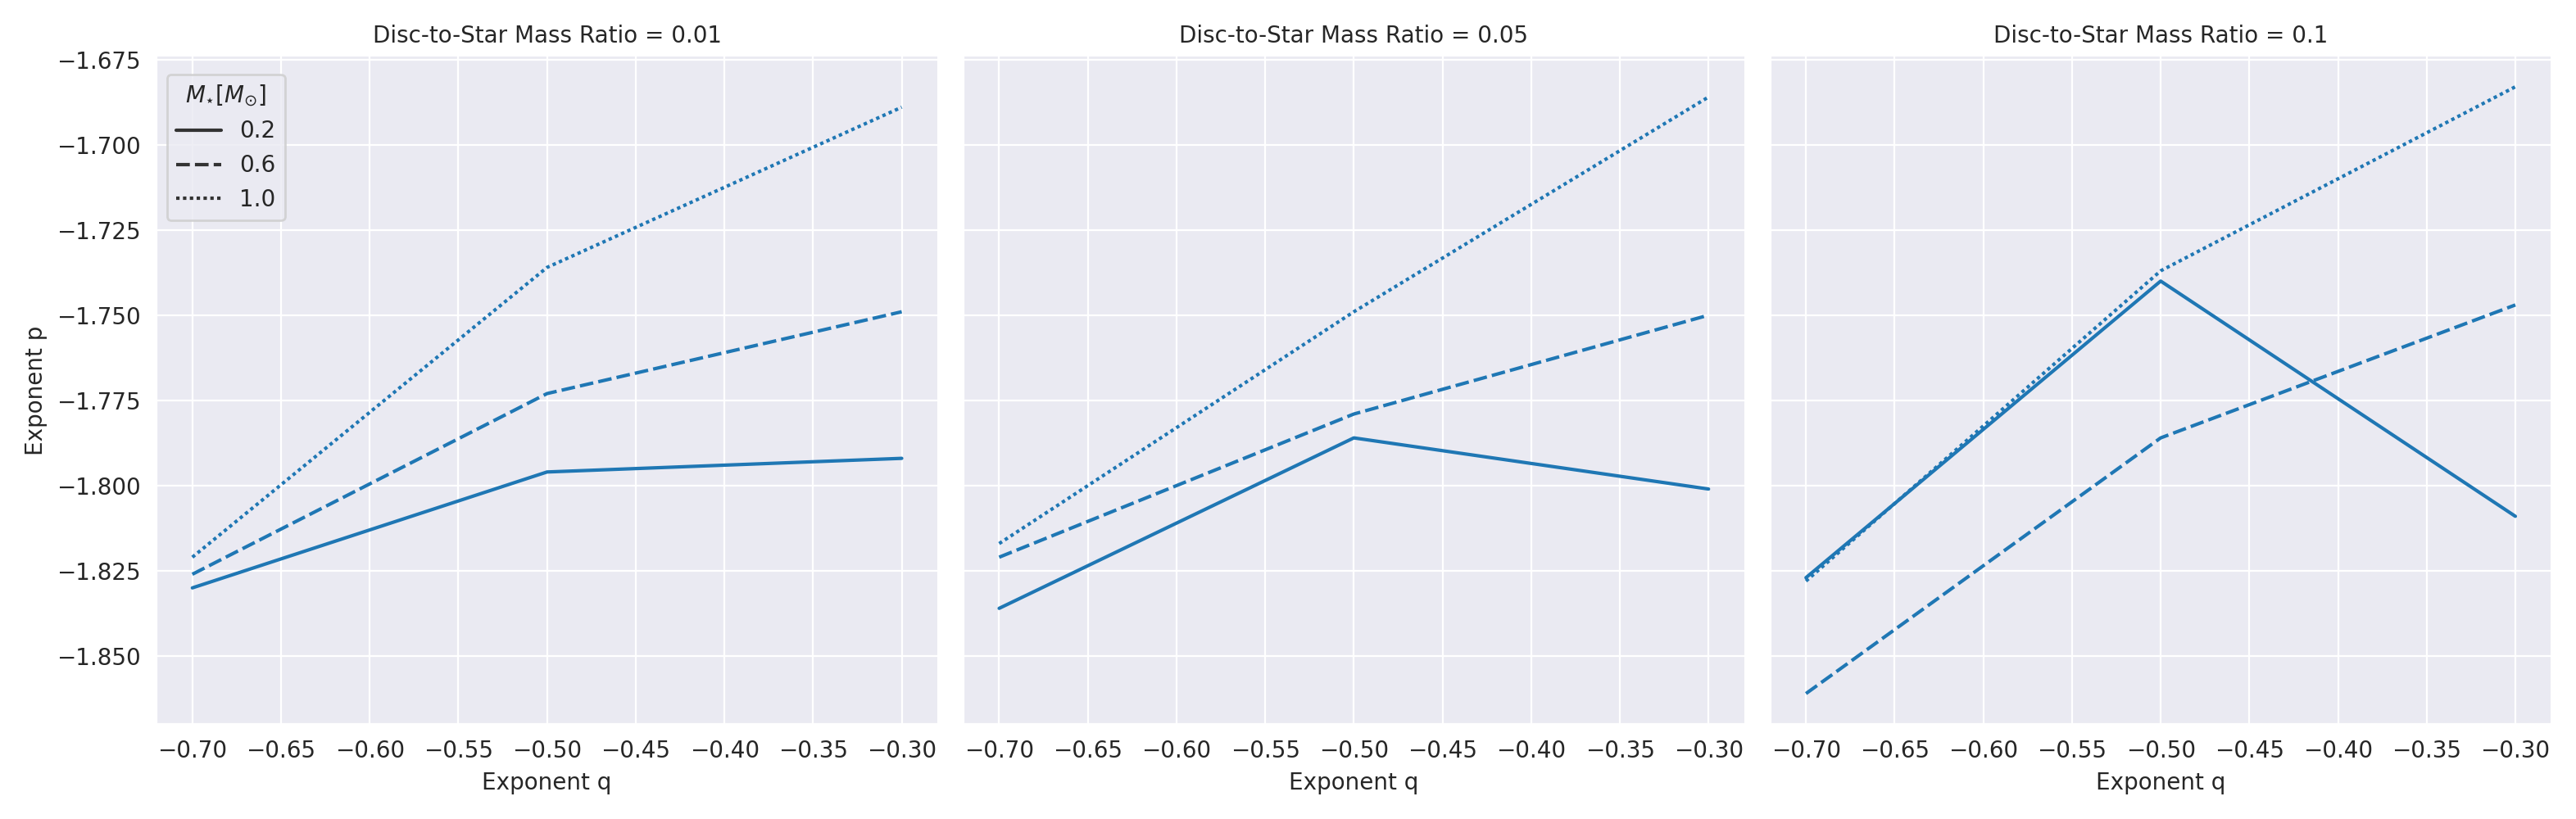
\includegraphics[width=\linewidth]{Figures/figure2.png}
    \caption{The exponent of the surface density profile of the disc in relation to the exponent of the temperature profile of the disc for different disc-to-star mass ratios}\label{fig:p vs q for different w}
\end{figure*}
\endgroup
\endgroup


\twocolumngrid
We first notice that at the beginning of each simulation the initial exponent of the surface density profile \eqref{eq:surface density} was set to $2.05$, while now our analysis concludes to $p \in [1.683, 1.861]$ (see \cref{tab:final slopes}). A lower $p$ corresponds to a flatter surface density profile, which means that the average velocity of gas particles was directed away from the central star, thus part of the gas has been moved to bigger values of $R$. Of course, a part of the gas was directed towards the central star and eventually accreted onto the star surface. The overall result depicts that in each case the redistribution of angular momentum within the disc leads to a less massive disc with a flatter surface density profile.

Furthermore, focusing on the simulations where the central star is more massive ($M_{\star} = 0.6 \; \& \; 1 M_{\odot}$) and simultaneously the disc is more massive (see \cref{tab:initial conditions}) we observe two things: first, as we choose steeper initial temperature profiles we conclude to also steeper surface density profiles (see \cref{fig:p vs q for different w}). The data implies that colder discs transfer angular momentum away more efficiently or equivalently that hotter discs transfer angular momentum away less efficiently. From \eqref{eq:height scale} and \eqref{eq:scale height self gravity} someone can notice that a colder disc corresponds to smaller height scale and from \eqref{eq:artificial viscosity} this leads to higher values of the Shakura \& Suynaev parameter $a_{SS}$. Consequently, the observed behavior of the disc evolution agrees with our theoretical models. Secondly, a more massive central star and simultaneously a more massive disc results to a flatter surface density profile. In our models, a more massive star means also a more luminous one \eqref{eq:mass-luminosity relation} and that corresponds to a hotter disc \eqref{eq:temperature-distance}. However, from \eqref{eq:height scale} and \eqref{eq:scale height self gravity} we notice that more massive systems (more massive stars and more massive discs) should have discs rotating faster, thus smaller height scales. The data implies that the contribution of the temperature is more important, but further simulations are necessary to receive safe results.

On the other hand, it is very interesting that in the case of the least massive central star ($M_{\star} = 0.2 \;  M_{\odot}$) the data implies not only that a colder disc does not necessarily transfer angular momentum away more efficiently, but also that a more massive central star and simultaneously a more massive disc does not necessarily result to a flatter surface density profile for the disc; The aforementioned discrepancy is evident in \cref{fig:p vs q for different w}, which also illustrates that this deviance becomes greater as the disc mass becomes greater.  It is possible that the 5000yr period is a small one for a simulation with such a low mass central star. As mentioned, less massive stars have discs rotating  slower, thus the disc around the $0.2M$ star does not necessarily completes  5  orbits. In that case, the disc may have not reached yet the equilibrium state. Further simulations are necessary to investigate in depth the behavior of discs around such low mass stars and to extract safe results.

\section{Conclusion and Discussion}
We used the SPH code ``PHANTOM'' to simulate isothermal gaseous protoplanetary discs evolving around low mass stars, while varying the disc-to-star mass ratio and the initial exponent of the temperature profile,$q$. For the most massive systems in our sample, where $M_{\star} = 0.6 \; \& \; 1 M_{\odot}$, we find that as we choose steeper initial temperature profile (colder disc) the transfer of angular momentum towards the limbs of the disc becomes more efficient resulting to steeper surface density profiles. By comparing now the different systems for the same $q$, the data hints that the more massive, which have more luminous stars based on our model, result to a flatter surface density profile. This implies that the temperature of the disc contributes more importantly than its rotational velocity to the transfer of angular momentum within the disc. Finally, the data do not allow us to safely assume that the aforementioned results also implied in the case of the least massive central star ($M_{\star} = 0.2 \;  M_{\odot}$).

In future work, more simulations would be necessary to provide further support and confirm that more massive systems, and simultaneously these with more luminous stars, result to flatter disc surface density profiles. Based on the data from the aforementioned simulations, a safer estimation on the importance of the temperature of the disc over its rotational velocity to the transfer of angular momentum within the disc would be possible. Finally, the discrepancy between the results for the least massive system ($M_{\star} = 0.2 \;  M_{\odot}$) and the rest systems ($M_{\star} = 0.6 \; \& \; 1 M_{\odot}$) seems very interesting. In this very low mass regime ($M_{\star} \sim 0.2 \;  M_{\odot}$), more simulations are necessary before we attempt to argue about the impact of the varying $q$ on the surface density profile of the disc after it has reached the equilibrium state.\par

\section{Acknowledgments}
I thank Dimitris Stamatellos for the guidance and the helpful discussions. I also thank Adam Fenton for the helpful discussions.

\begin{table}[!htbp]
  \centering
  \setlength{\tabcolsep}{12pt} % Default value: 6pt
  \begin{tabular}{cccc}
  \hline
  $Run$ & $p$ &  $\Sigma_0 \; (g/cm^2)$ & $q$ \\
  \hline \hline
  1 & 1.792 $\pm$ 0.014 & 514 $\pm$ 24.11 & 0.3\\
  2 & 1.796 $\pm$ 0.013 & 533 $\pm$ 23.24 & 0.5 \\
  3 & 1.830 $\pm$ 0.013 & 622 $\pm$ 26.68 & 0.7 \\
  \hline
  4 & 1.801 $\pm$ 0.013 & 2616 $\pm$ 104.64 & 0.3 \\
  5 & 1.786 $\pm$ 0.016 & 2535 $\pm$ 131.31 & 0.5 \\
  6 & 1.836 $\pm$ 0.014 & 3110 $\pm$ 139.33 & 0.7 \\
  \hline
  7 & 1.809 $\pm$ 0.016 & 5263 $\pm$ 257.25 & 0.3 \\
  8 & 1.740 $\pm$ 0.017 & 3875 $\pm$ 218.55 & 0.5 \\
  9 & 1.827 $\pm$ 0.012 & 5934 $\pm$ 232.61 & 0.7 \\
  \hline
  10 & 1.749 $\pm$ 0.017 & 1358 $\pm$ 74.28 & 0.3 \\
  11 & 1.773 $\pm$ 0.013 & 1526 $\pm$ 66.23 & 0.5 \\
  12 & 1.826 $\pm$ 0.012 & 1868 $\pm$ 73.60 & 0.7 \\
  \hline
  13 & 1.750 $\pm$ 0.014 & 6689 $\pm$ 318.40 & 0.3 \\
  14 & 1.779 $\pm$ 0.014 & 7668 $\pm$ 361.93 & 0.5 \\
  15 & 1.821 $\pm$ 0.013 & 9043 $\pm$ 377.09 & 0.7 \\
  \hline
  16 & 1.747 $\pm$ 0.014 & 13019 $\pm$ 583.25 & 0.3 \\
  17 & 1.786 $\pm$ 0.013 & 15491 $\pm$ 647.52 & 0.5 \\
  18 & 1.861 $\pm$ 0.013 & 20621 $\pm$ 853.71 & 0.7 \\
  \hline
  19 & 1.689 $\pm$ 0.016 & 1816 $\pm$ 94.432 & 0.3 \\
  20 & 1.736 $\pm$ 0.015 & 2251 $\pm$ 111.65 & 0.5 \\
  21 & 1.821 $\pm$ 0.011 & 3070 $\pm$ 115.74 & 0.7 \\
  \hline
  22 & 1.686 $\pm$ 0.017 & 8861 $\pm$ 483.81 & 0.3 \\
  23 & 1.749 $\pm$ 0.014 & 11545 $\pm$ 544.92 & 0.5 \\
  24 & 1.817 $\pm$ 0.012 & 14999 $\pm$ 590.96 & 0.7 \\
  \hline
  25 & 1.683 $\pm$ 0.017 & 17281 $\pm$ 969.46 & 0.3 \\
  26 & 1.737 $\pm$ 0.015 & 21821 $\pm$ 1108.50 & 0.5 \\
  27 & 1.828 $\pm$ 0.013 & 30526 $\pm$ 1327.88 & 0.7 \\
  \hline
 \end{tabular}
\caption{The parameters of the surface density profile and the initial slope of the temperature profile of each simulation}\label{tab:final slopes}
\end{table}

\begin{comment}
\clearpage
\onecolumngrid
\begingroup
\begin{table*}[!htbp]
  \centering
  \setlength{\tabcolsep}{12pt} % Default value: 6pt
  \begin{tabular}{cccc}
  \hline
  $Run$ & $p$ &  $\Sigma_0 \; (g/cm^2)$ & $q$ \\
  \hline \hline
  1 & 1.792 $\pm$ 0.014 & 514 $\pm$ 24.11 & 0.3\\
  2 & 1.796 $\pm$ 0.013 & 533 $\pm$ 23.24 & 0.5 \\
  3 & 1.830 $\pm$ 0.013 & 622 $\pm$ 26.68 & 0.7 \\
  \hline
  4 & 1.801 $\pm$ 0.013 & 2616 $\pm$ 104.64 & 0.3 \\
  5 & 1.786 $\pm$ 0.016 & 2535 $\pm$ 131.31 & 0.5 \\
  6 & 1.836 $\pm$ 0.014 & 3110 $\pm$ 139.33 & 0.7 \\
  \hline
  7 & 1.809 $\pm$ 0.016 & 5263 $\pm$ 257.25 & 0.3 \\
  8 & 1.740 $\pm$ 0.017 & 3875 $\pm$ 218.55 & 0.5 \\
  9 & 1.827 $\pm$ 0.012 & 5934 $\pm$ 232.61 & 0.7 \\
  \hline
  10 & 1.749 $\pm$ 0.017 & 1358 $\pm$ 74.28 & 0.3 \\
  11 & 1.773 $\pm$ 0.013 & 1526 $\pm$ 66.23 & 0.5 \\
  12 & 1.826 $\pm$ 0.012 & 1868 $\pm$ 73.60 & 0.7 \\
  \hline
  13 & 1.750 $\pm$ 0.014 & 6689 $\pm$ 318.40 & 0.3 \\
  14 & 1.779 $\pm$ 0.014 & 7668 $\pm$ 361.93 & 0.5 \\
  15 & 1.821 $\pm$ 0.013 & 9043 $\pm$ 377.09 & 0.7 \\
  \hline
  16 & 1.747 $\pm$ 0.014 & 13019 $\pm$ 583.25 & 0.3 \\
  17 & 1.786 $\pm$ 0.013 & 15491 $\pm$ 647.52 & 0.5 \\
  18 & 1.861 $\pm$ 0.013 & 20621 $\pm$ 853.71 & 0.7 \\
  \hline
  19 & 1.689 $\pm$ 0.016 & 1816 $\pm$ 94.432 & 0.3 \\
  20 & 1.736 $\pm$ 0.015 & 2251 $\pm$ 111.65 & 0.5 \\
  21 & 1.821 $\pm$ 0.011 & 3070 $\pm$ 115.74 & 0.7 \\
  \hline
  22 & 1.686 $\pm$ 0.017 & 8861 $\pm$ 483.81 & 0.3 \\
  23 & 1.749 $\pm$ 0.014 & 11545 $\pm$ 544.92 & 0.5 \\
  24 & 1.817 $\pm$ 0.012 & 14999 $\pm$ 590.96 & 0.7 \\
  \hline
  25 & 1.683 $\pm$ 0.017 & 17281 $\pm$ 969.46 & 0.3 \\
  26 & 1.737 $\pm$ 0.015 & 21821 $\pm$ 1108.50 & 0.5 \\
  27 & 1.828 $\pm$ 0.013 & 30526 $\pm$ 1327.88 & 0.7 \\
  \hline
 \end{tabular}
\caption{The parameters of the surface density profile and the initial slope of the temperature profile of each simulation}\label{tab:final slopes}
\end{table*}
\endgroup
\end{comment}

\clearpage
\begin{appendices}
\crefalias{section}{appendix}
\onecolumngrid

\section{- Azimuthally-averaged surface density profiles}\label{app:appendixA}
\begin{figure*}[!htbp]\vspace*{4cm}
  \centering
    \subcaptionbox*{}[.32\linewidth][c]{%
    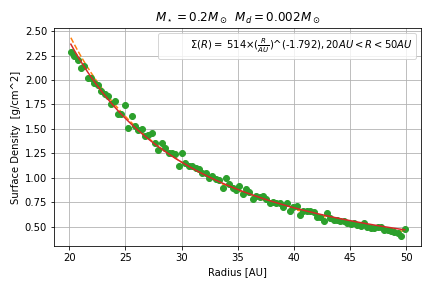
\includegraphics[width=\linewidth]{Graphs_1D/r_0.2s_0.002d_0.3q_1D.png}}\quad
    \vspace{-2\baselineskip}
  \subcaptionbox*{}[.32\linewidth][c]{%
    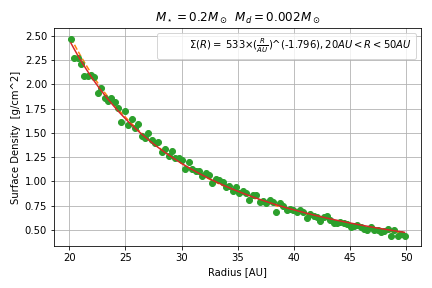
\includegraphics[width=\linewidth]{Graphs_1D/r_0.2s_0.002d_0.5q_1D.png}}\quad
  \subcaptionbox*{}[.32\linewidth][c]{%
    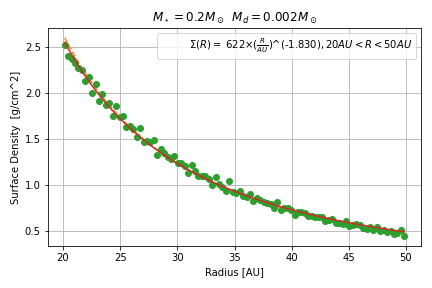
\includegraphics[width=\linewidth]{Graphs_1D/r_0.2s_0.002d_0.7q_1D.png}}\quad
  \subcaptionbox*{}[.32\linewidth][c]{%
    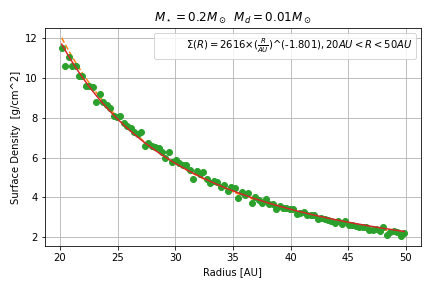
\includegraphics[width=\linewidth]{Graphs_1D/r_0.2s_0.01d_0.3q_1D.png}}\quad
    \vspace{-2\baselineskip}
  \subcaptionbox*{}[.32\linewidth][c]{%
    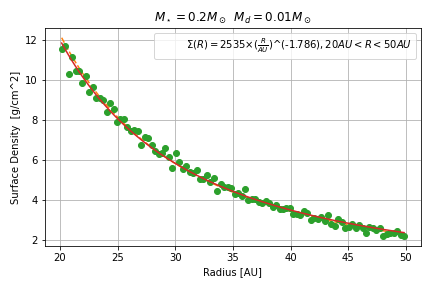
\includegraphics[width=\linewidth]{Graphs_1D/r_0.2s_0.01d_0.5q_1D.png}}\quad
  \subcaptionbox*{}[.32\linewidth][c]{%
    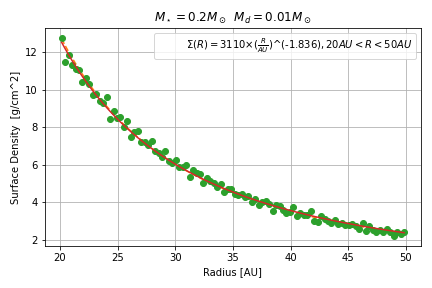
\includegraphics[width=\linewidth]{Graphs_1D/r_0.2s_0.01d_0.7q_1D.png}}\quad
  \subcaptionbox*{}[.32\linewidth][c]{%
     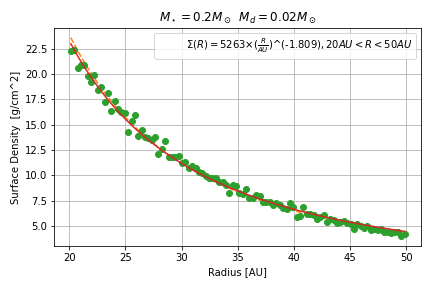
\includegraphics[width=\linewidth]{Graphs_1D/r_0.2s_0.02d_0.3q_1D.png}}\quad
     \vspace{-2\baselineskip}
  \subcaptionbox*{}[.32\linewidth][c]{%
    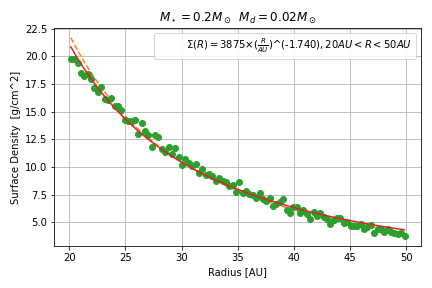
\includegraphics[width=\linewidth]{Graphs_1D/r_0.2s_0.02d_0.5q_1D.png}}\quad
  \subcaptionbox*{}[.32\linewidth][c]{%
    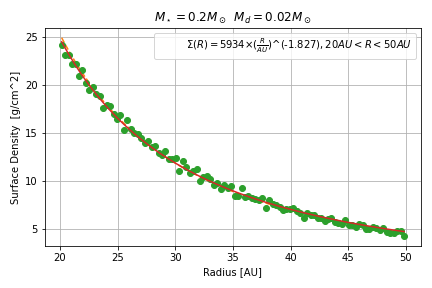
\includegraphics[width=\linewidth]{Graphs_1D/r_0.2s_0.02d_0.7q_1D.png}}\quad
  \caption{1-D Illustrations of the surface density profile of the disc around a $0.2 M_{\odot}$ star after $5000yr$. The disc-to-star mass ratio equals to $0.01, 0.05, 0.1$ for each row respectively, while the initial slope of the temperature profile of the disc equals to $0.3, 0.5, 0.7$ for each column respectively. The disc has reached its relaxed state and the slope of surface density profile has been stabilized. The dashed line show the initial conditions for the fit.}
\end{figure*}

\begin{figure*}[!htbp]\vspace*{4cm}
  \centering
  \subcaptionbox*{}[.32\linewidth][c]{%
    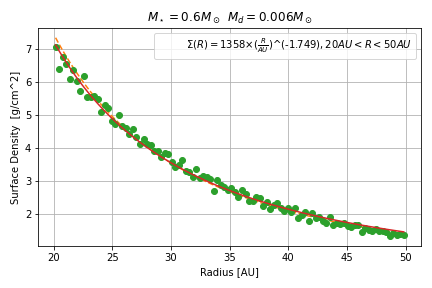
\includegraphics[width=\linewidth]{Graphs_1D/r_0.6s_0.006d_0.3q_1D.png}}\quad
  \subcaptionbox*{}[.32\linewidth][c]{%
    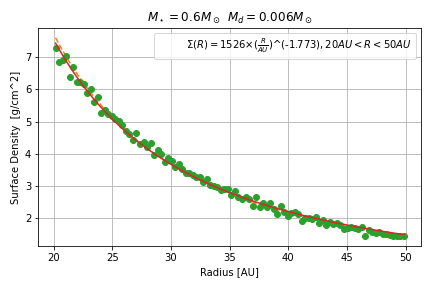
\includegraphics[width=\linewidth]{Graphs_1D/r_0.6s_0.006d_0.5q_1D.png}}\quad
  \subcaptionbox*{}[.32\linewidth][c]{%
    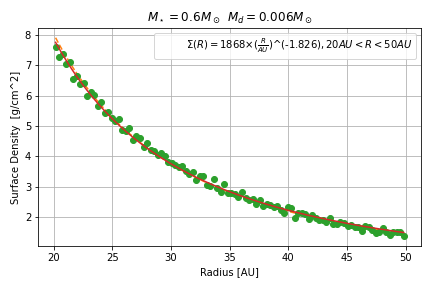
\includegraphics[width=\linewidth]{Graphs_1D/r_0.6s_0.006d_0.7q_1D.png}}\quad
  \subcaptionbox*{}[.32\linewidth][c]{%
    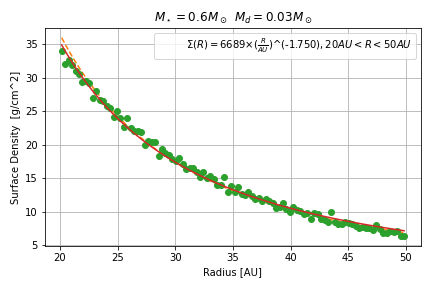
\includegraphics[width=\linewidth]{Graphs_1D/r_0.6s_0.03d_0.3q_1D.png}}\quad
  \subcaptionbox*{}[.32\linewidth][c]{%
    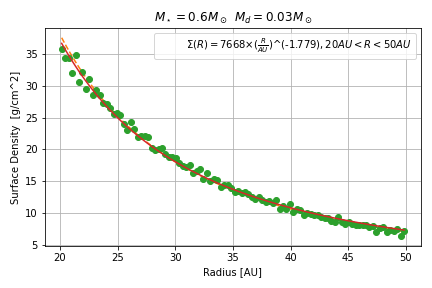
\includegraphics[width=\linewidth]{Graphs_1D/r_0.6s_0.03d_0.5q_1D.png}}\quad
  \subcaptionbox*{}[.32\linewidth][c]{%
    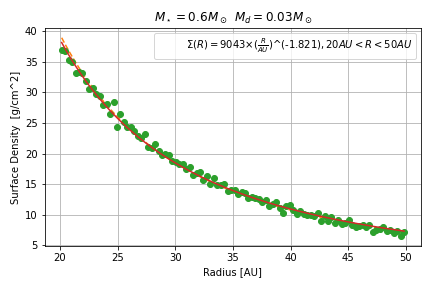
\includegraphics[width=\linewidth]{Graphs_1D/r_0.6s_0.03d_0.7q_1D.png}}\quad    
  \subcaptionbox*{}[.32\linewidth][c]{%
    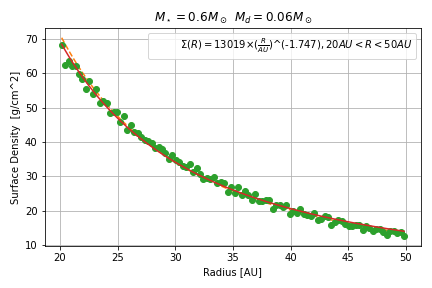
\includegraphics[width=\linewidth]{Graphs_1D/r_0.6s_0.06d_0.3q_1D.png}}\quad
  \subcaptionbox*{}[.32\linewidth][c]{%
    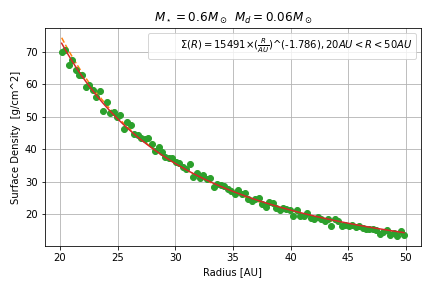
\includegraphics[width=\linewidth]{Graphs_1D/r_0.6s_0.06d_0.5q_1D.png}}\quad
  \subcaptionbox*{}[.32\linewidth][c]{%
    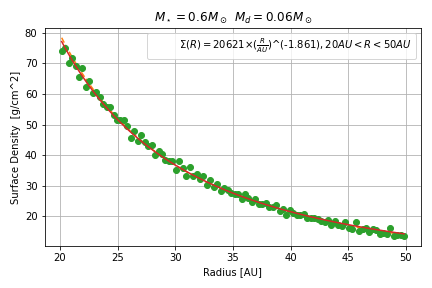
\includegraphics[width=\linewidth]{Graphs_1D/r_0.6s_0.06d_0.7q_1D.png}}\quad
  \caption{1-D Illustrations of the surface density profile of the disc around a $0.6 M_{\odot}$ star after $5000yr$. The disc-to-star mass ratio equals to $0.01, 0.05, 0.1$ for each row respectively, while the initial slope of the temperature profile of the disc equals to $0.3, 0.5, 0.7$ for each column respectively. The disc has reached its relaxed state and the slope of surface density profile has been stabilized. The dashed line show the initial conditions for the fit.}
\end{figure*}
  
\begin{figure*}[!htbp]\vspace*{4cm}
  \centering
  \subcaptionbox*{}[.32\linewidth][c]{%
    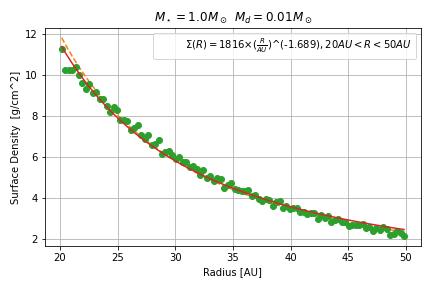
\includegraphics[width=\linewidth]{Graphs_1D/r_1s_0.01d_0.3q_1D.png}}\quad
  \subcaptionbox*{}[.32\linewidth][c]{%
    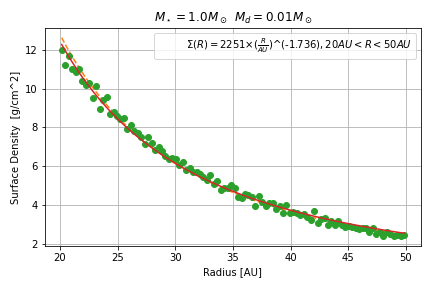
\includegraphics[width=\linewidth]{Graphs_1D/r_1s_0.01d_0.5q_1D.png}}\quad
  \subcaptionbox*{}[.32\linewidth][c]{%
    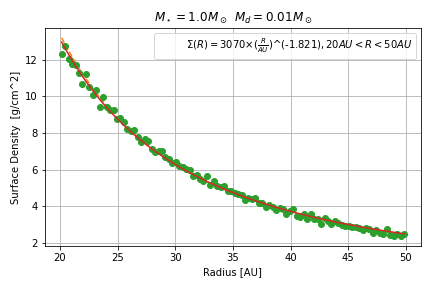
\includegraphics[width=\linewidth]{Graphs_1D/r_1s_0.01d_0.7q_1D.png}}\quad
  \subcaptionbox*{}[.32\linewidth][c]{%
    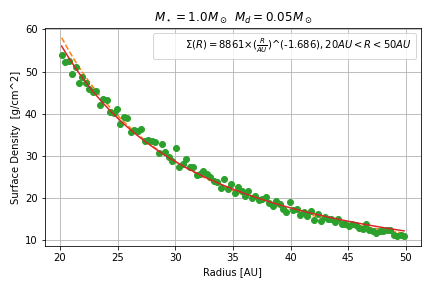
\includegraphics[width=\linewidth]{Graphs_1D/r_1s_0.05d_0.3q_1D.png}}\quad
  \subcaptionbox*{}[.32\linewidth][c]{%
    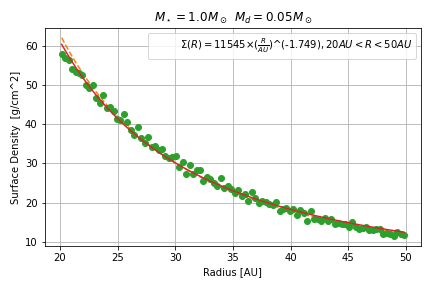
\includegraphics[width=\linewidth]{Graphs_1D/r_1s_0.05d_0.5q_1D.png}}\quad
  \subcaptionbox*{}[.32\linewidth][c]{%
    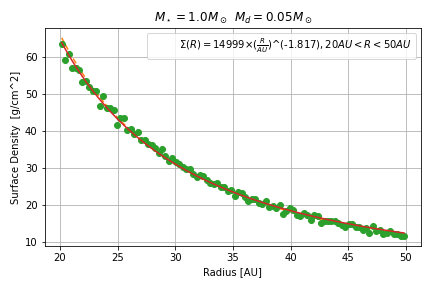
\includegraphics[width=\linewidth]{Graphs_1D/r_1s_0.05d_0.7q_1D.png}}\quad  
  \subcaptionbox*{}[.32\linewidth][c]{%
    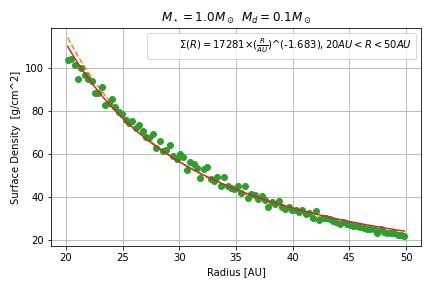
\includegraphics[width=\linewidth]{Graphs_1D/r_1s_0.1d_0.3q_1D.png}}\quad
  \subcaptionbox*{}[.32\linewidth][c]{%
    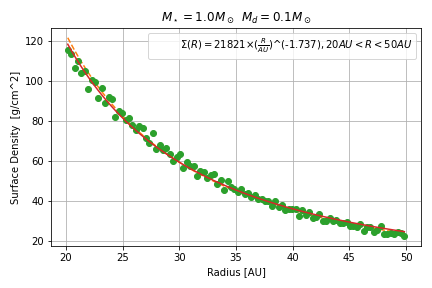
\includegraphics[width=\linewidth]{Graphs_1D/r_1s_0.1d_0.5q_1D.png}}\quad
  \subcaptionbox*{}[.32\linewidth][c]{%
    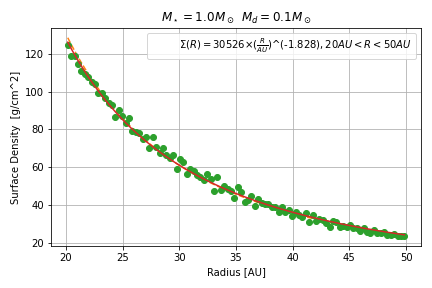
\includegraphics[width=\linewidth]{Graphs_1D/r_1s_0.1d_0.7q_1D.png}}\quad
  \caption{1-D Illustrations of the surface density profile of the disc around a $1 M_{\odot}$ star after $5000yr$. The disc-to-star mass ratio equals to $0.01, 0.05, 0.1$ for each row respectively, while the initial slope of the temperature profile of the disc equals to $0.3, 0.5, 0.7$ for each column respectively. The disc has reached its relaxed state and the slope of surface density profile has been stabilized. The dashed line show the initial conditions for the fit.}
\end{figure*} 
\clearpage
\section{- Disc Surface Density}\label{app:appendixB}
\begin{figure*}[!htbp]\vspace*{3cm}
  \centering
   \subcaptionbox*{}[.32\linewidth][c]{%
      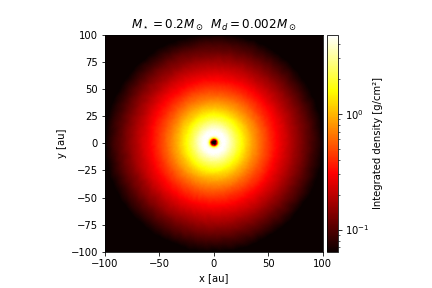
\includegraphics[width=\linewidth]{Graphs_2D/r_0.2s_0.002d_0.3q_2D.png}}\quad
      \vspace{-2\baselineskip}
  \subcaptionbox*{}[.32\linewidth][c]{%
    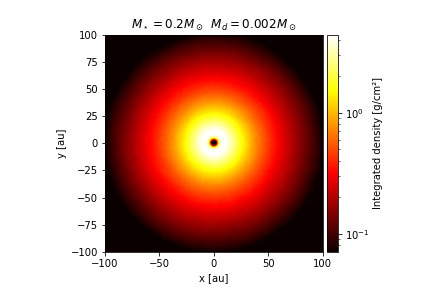
\includegraphics[width=\linewidth]{Graphs_2D/r_0.2s_0.002d_0.5q_2D.png}}\quad
  \subcaptionbox*{}[.32\linewidth][c]{%
    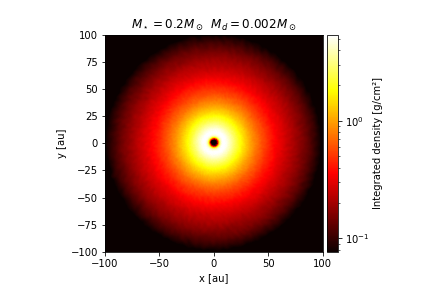
\includegraphics[width=\linewidth]{Graphs_2D/r_0.2s_0.002d_0.7q_2D.png}}\quad
  \subcaptionbox*{}[.32\linewidth][c]{%
    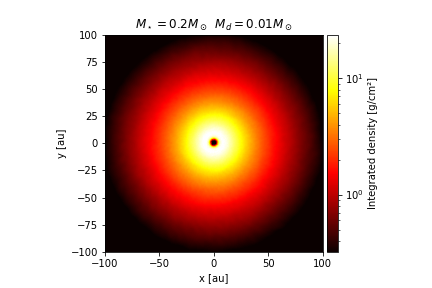
\includegraphics[width=1\linewidth]{Graphs_2D/r_0.2s_0.01d_0.3q_2D.png}}\quad
    \vspace{-2\baselineskip}
  \subcaptionbox*{}[.32\linewidth][c]{%
    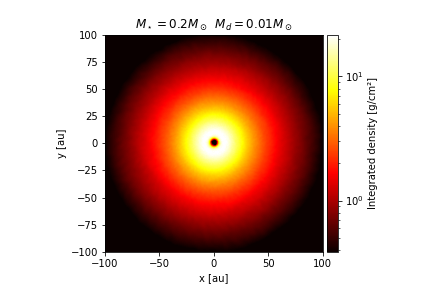
\includegraphics[width=\linewidth]{Graphs_2D/r_0.2s_0.01d_0.5q_2D.png}}\quad
  \subcaptionbox*{}[.32\linewidth][c]{%
    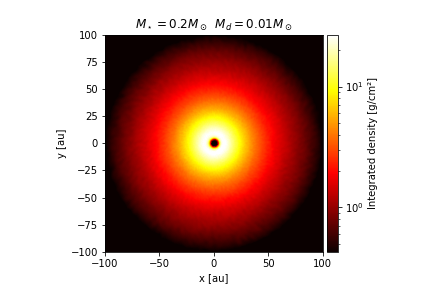
\includegraphics[width=\linewidth]{Graphs_2D/r_0.2s_0.01d_0.7q_2D.png}}\quad 
  \subcaptionbox*{}[.32\linewidth][c]{%
    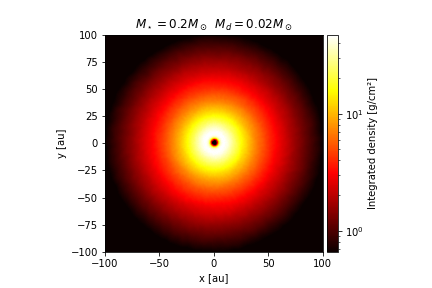
\includegraphics[width=\linewidth]{Graphs_2D/r_0.2s_0.02d_0.3q_2D.png}}\quad
    \vspace{-2\baselineskip}
  \subcaptionbox*{}[.32\linewidth][c]{%
    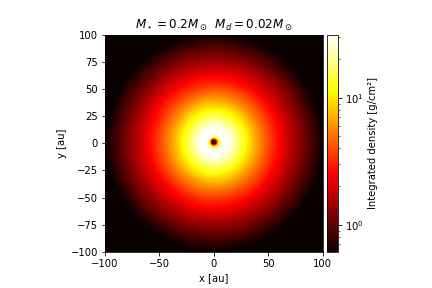
\includegraphics[width=\linewidth]{Graphs_2D/r_0.2s_0.02d_0.5q_2D.png}}\quad
  \subcaptionbox*{}[.32\linewidth][c]{%
    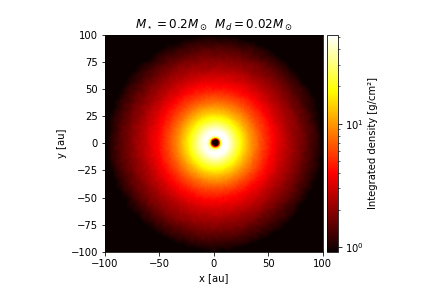
\includegraphics[width=\linewidth]{Graphs_2D/r_0.2s_0.02d_0.7q_2D.png}}\quad
  \caption{2-D Illustrations of the surface density of the disc around a $0.2 M_{\odot}$ star after $5000yr$ - colorbar in logarithmic scale. The disc-to-star mass ratio equals to $0.01, 0.05, 0.1$ for each row respectively, while the initial slope of the temperature profile of the disc equals to $0.3, 0.5, 0.7$ for each column respectively. The disc has reached its relaxed state and the slope of surface density profile has been stabilized}
\end{figure*}
 
\begin{figure*}[!htbp]\vspace*{3cm}
  \centering
  \subcaptionbox*{}[.32\linewidth][c]{%
    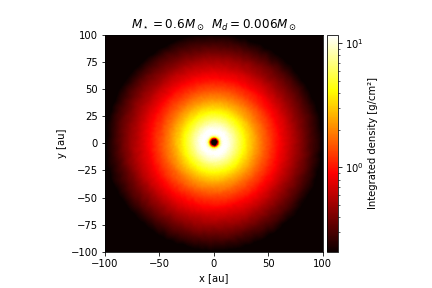
\includegraphics[width=\linewidth]{Graphs_2D/r_0.6s_0.006d_0.3q_2D.png}}\quad
  \subcaptionbox*{}[.32\linewidth][c]{%
    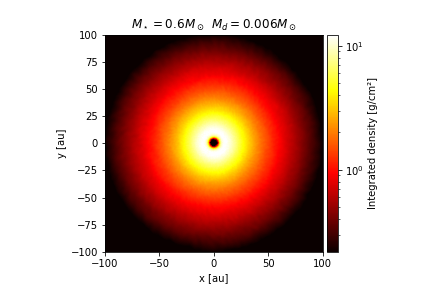
\includegraphics[width=\linewidth]{Graphs_2D/r_0.6s_0.006d_0.5q_2D.png}}\quad
  \subcaptionbox*{}[.32\linewidth][c]{%
    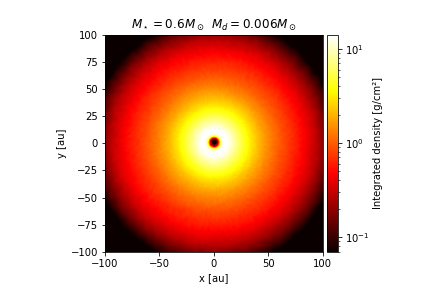
\includegraphics[width=\linewidth]{Graphs_2D/r_0.6s_0.006d_0.7q_2D.png}}\quad
  \subcaptionbox*{}[.32\linewidth][c]{%
    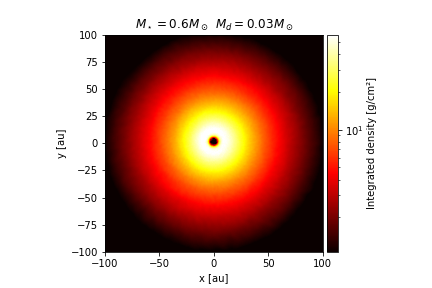
\includegraphics[width=1\linewidth]{Graphs_2D/r_0.6s_0.03d_0.3q_2D.png}}\quad
  \subcaptionbox*{}[.32\linewidth][c]{%
    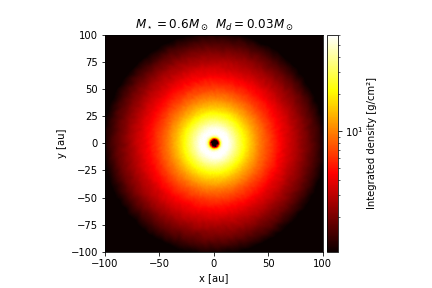
\includegraphics[width=\linewidth]{Graphs_2D/r_0.6s_0.03d_0.5q_2D.png}}\quad
  \subcaptionbox*{}[.32\linewidth][c]{%
    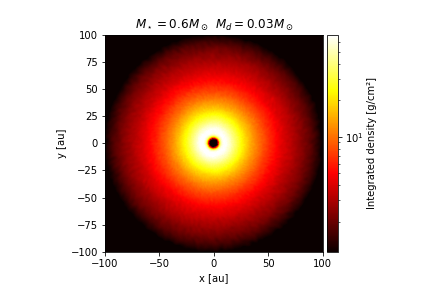
\includegraphics[width=\linewidth]{Graphs_2D/r_0.6s_0.03d_0.7q_2D.png}}\quad    
  \subcaptionbox*{}[.32\linewidth][c]{%
    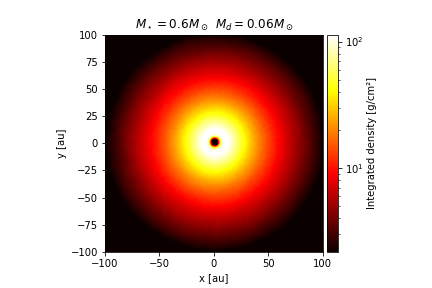
\includegraphics[width=\linewidth]{Graphs_2D/r_0.6s_0.06d_0.3q_2D.png}}\quad
  \subcaptionbox*{}[.32\linewidth][c]{%
    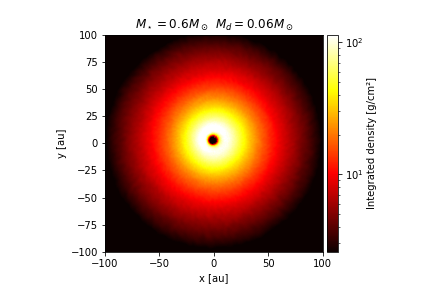
\includegraphics[width=\linewidth]{Graphs_2D/r_0.6s_0.06d_0.5q_2D.png}}\quad
  \subcaptionbox*{}[.32\linewidth][c]{%
    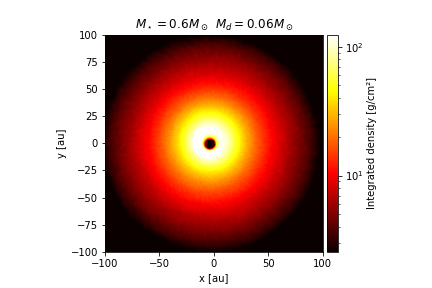
\includegraphics[width=\linewidth]{Graphs_2D/r_0.6s_0.06d_0.7q_2D.png}}\quad
  \caption{2-D Illustrations of the surface density of the disc around a $0.6 M_{\odot}$ star after $5000yr$ - colorbar in logarithmic scale. The disc-to-star mass ratio equals to $0.01, 0.05, 0.1$ for each row respectively, while the initial slope of temperature profile of the disc equals to $0.3, 0.5, 0.7$ for each column respectively. The disc has reached its relaxed state and the slope of surface density profile has been stabilized}
\end{figure*}

\begin{figure*}[!htbp]\vspace*{3cm}
  \centering
  \subcaptionbox*{}[.32\linewidth][c]{%
    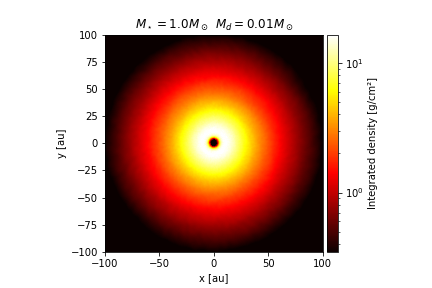
\includegraphics[width=\linewidth]{Graphs_2D/r_1s_0.01d_0.3q_2D.png}}\quad
  \subcaptionbox*{}[.32\linewidth][c]{%
    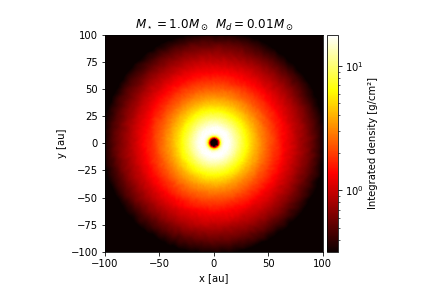
\includegraphics[width=\linewidth]{Graphs_2D/r_1s_0.01d_0.5q_2D.png}}\quad
  \subcaptionbox*{}[.32\linewidth][c]{%
    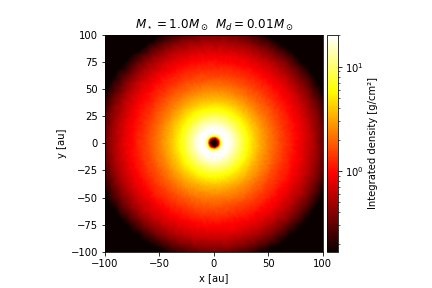
\includegraphics[width=\linewidth]{Graphs_2D/r_1s_0.01d_0.7q_2D.png}}\quad
  \subcaptionbox*{}[.32\linewidth][c]{%
    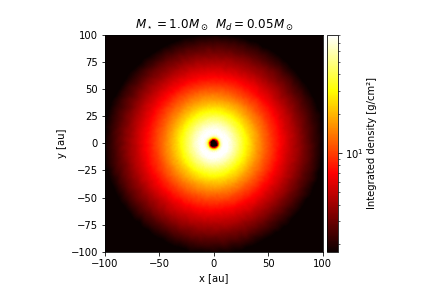
\includegraphics[width=1\linewidth]{Graphs_2D/r_1s_0.05d_0.3q_2D.png}}\quad
  \subcaptionbox*{}[.32\linewidth][c]{%
    \includegraphics[width=\linewidth]{Graphs_2D/r_1s_0.05d_0.5q_2D.png}}\quad
  \subcaptionbox*{}[.32\linewidth][c]{%
    \includegraphics[width=\linewidth]{Graphs_2D/r_1s_0.05d_0.7q_2D.png}}\quad    
  \subcaptionbox*{}[.32\linewidth][c]{%
    \includegraphics[width=\linewidth]{Graphs_2D/r_1s_0.1d_0.3q_2D.png}}\quad
  \subcaptionbox*{}[.32\linewidth][c]{%
    \includegraphics[width=\linewidth]{Graphs_2D/r_1s_0.1d_0.5q_2D.png}}\quad
  \subcaptionbox*{}[.32\linewidth][c]{%
    \includegraphics[width=\linewidth]{Graphs_2D/r_1s_0.1d_0.7q_2D.png}}\quad
  \caption{2-D Illustrations of the surface density of the disc around a $1 M_{\odot}$ star after $5000yr$ - colorbar in logarithmic scale. The disc-to-star mass ratio equals to $0.01, 0.05, 0.1$ for each row respectively, while the initial slope of the temperature profile of the disc equals to $0.3, 0.5, 0.7$ for each column respectively. The disc has reached its relaxed state and the slope of surface density profile has been stabilized}
\end{figure*}
\end{appendices}
\newpage
\twocolumngrid
\clearpage
\setcitestyle{numbers}
\bibliographystyle{plainnat}
\bibliography{bibliography}
\end{document}
